\section{IIC-Bus}

\subsection{IIC-Bus Properties}

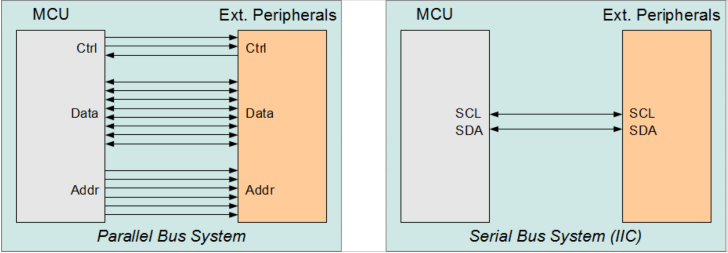
\includegraphics[width=0.5\textwidth]{iic-bus-wire.png}

\begin{itemize}
    \item{
        \textit{
            2 bidirectional wires (Clock: \textbf{SCL}, Data: \textbf{SDA})
        }
    }
    \item{
        \textit{
            Clock rates: \textbf{Standard 100 kHz; Fast 400 kHz}; Fast Plus 1 MHz;
            High Speed 3,4 MHz
        }
    }
    \item{
        \textit{
            Master/Slave-architecture, multiple masters are possible (\textbf{Bus Arbiter})
        }
    }
    \item{
        \textit{
            Number of participants is limited by number of addresses and wire capacity
        }
    }
    \item{
        \textit{
            Bus participants of different speeds are possible (\textbf{Clock Stretching}).
            Clock Stretching enables the slave to slow down the master.
        }
    }
\end{itemize}

\subsection{IIC-Bus stages}

\begin{itemize}
    \item{
        \textit{
            All bus participants use \textbf{Open-Drain Output stages}
            (no active H-Level possible).
        }
    }
    \item{
        \textit{
            \textbf{External Pullup}-Resistors generate the H-Level (Default-State).
        }
    }
    \item{
        \textit{
            All bus participants observe at all times the actual state of SCL (Clock) and SDA (Data).
        }
    }
\end{itemize}

\textit{
    \textbf{IIC without hardware support:}\newline
    If the IIC is not supported by the hardware, the open drain
    can be simulated. This is possible by setting the pins Internal
    pullup to 1 (PTxPEn = 1). Set the Output to 0 (PTxDn = 0). To write 1 (PTxDDn = 0)
    and 0 (PTxDDn = 1) use the datadirection. This will prevent any short circuits.
}

\subsection{Bit-Transfer}

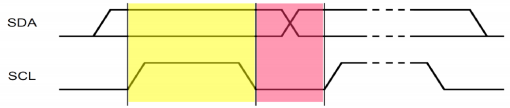
\includegraphics[width=0.5\textwidth]{iic-bit-transfer.png}

\textit{
    SDA (Data) can be changed if SCL=0, \newline
    and is evaluated when SCL=1.
}

\subsection{Start-/Stop-Condition}

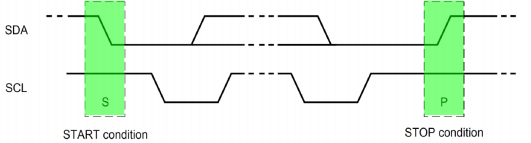
\includegraphics[width=0.5\textwidth]{iic-start-stop.png}

\textit{
    \textbf{Start-/Stop}-Conditions are always generated by the Master.
    As \textbf{protocol mismatch} they are detected by other Masters and
    Slaves and can easily be differenciated from normal data bits.
    \newline
}
\textit{
    \textbf{After} a \textbf{Start}-Condition, the bus is \textbf{busy}. \newline
}
\textit{
    \textbf{After} a \textbf{Stop}-Condition, the bus is \textbf{idle}.
}

\subsection{Byte Transfer (Blocks)}

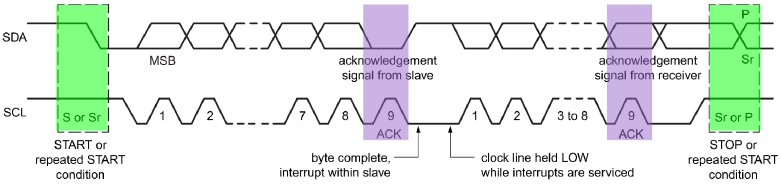
\includegraphics[width=0.5\textwidth]{iic-byte-transfer.png}

\begin{itemize}
    \item{
        \textit{
            Data transmission from transmitter to receiver is \textbf{Byte-wise} (\textbf{MSB-first}).
        }
    }
    \item{
        \textit{
            At the end of each byte, the \textbf{Receiver} generates an Acknowledge-Bit:
        }
        \begin{tabular}{cc}
            \textbf{SDA = 0 = Ack} & \textbf{SDA = 1 = No-Ack} \\
        \end{tabular}
        \textit{
            Through the generation of No-Ack, a transfer can be cancelled (premature).
        }
    }
    \item{
        \textit{
            A \textbf{Repeated-Start} (Sr) Condition can be generated by the active Master
            instead of a Stop-Condition, if the Master wants to continually use the bus
        }
    }
    \item{
        \textit{
            A Slave can force a Master to slow transmission through \textbf{Clock Stretching}.
        }
    }
\end{itemize}

\subsection{Slave Addressing}

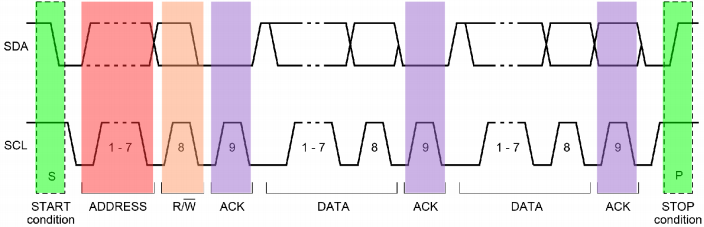
\includegraphics[width=0.5\textwidth]{iic-slave-addressing.png}

\begin{itemize}
    \item{
        \textit{
            In the first byte after the Start-Condition the master sends a \textbf{7-Bit
            Address}.
        }
    }
    \item{
        \textit{
            A slave with this address has to answer in the 9th bit with an Ack-Signal.
        }
    }
    \item{
        \textit{
            In the \textbf{8th bit} the master sends the \textbf{R/W} direction-bit: \newline
            \textbf{R/W = 0} : Write : Master-Transmitter to Slave-Receiver \newline
            \textbf{R/W = 1} : Read : Master-Receiver from Slave-Transmitter
        }
    }
    \item{
        \textit{
            Combined R/W Transfer-formats are possible through Repeated-Start
            Condition.
        }
    }
\end{itemize}

\subsection{Function Schema \& Control Register}

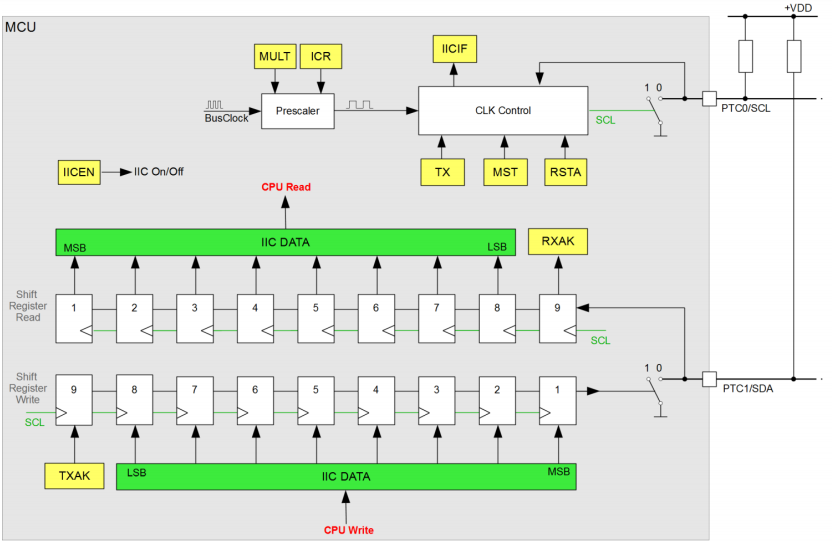
\includegraphics[width=0.5\textwidth]{iic-schema.png}

\begin{tabular}{ll}
    \textbf{IICEN}: Block enable & \textbf{IICIE}: Interrupt en. \\
    \textbf{MST}: master \& busy & \textbf{Tx}: transmit \\
    \textbf{TXAK}: ack enable    & \textbf{RSTA}: repeat start \\
                                 & $f_{IIC} = f_{BUS} / MULTxf(ICR)$ \\
    \textbf{TCF}: transfer done  & \textbf{IAAS}: addressed \\
    \textbf{BUSY}: bus busy      & \textbf{ARBL}: arbitration lost \\
    \textbf{SRW}: slave R/W      & \textbf{IICIF}: int. Flag \\
    \textbf{RXAK}: acknowledged  & \\
\end{tabular}

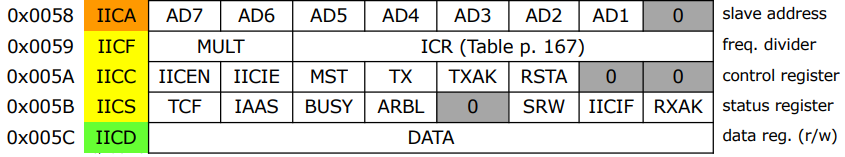
\includegraphics[width=0.5\textwidth]{iic-control-register.png}

\begin{itemize}
    \item{
        \textit{
            IICD: 7 Bit Daten, 1 Bit R/W
        }
    }
    \item{
        \textit{
            IICS\_IICIF: IIC Interrupt Flag wird gesetzt wenn: 1Byte transferiert wurde,
            Slave Adresse und angesprochene Adresse identisch sind oder Arbitration lost.
        }
    }
    \item{
        \textit{
            IICS\_RXAK: 0=Acknowlage recieved, 1=no Achnowlage recieved.
        }
    }
    \item{
        \textit{
            IICC\_MST: wechsel von 0 nach 1 generiert Stop.
        }
    }
    \item{
        \textit{
            IICS\_IICIF: =1 resetet den Interrupt.
        }
    }
    \item{
        \textit{
            IICC\_TSAK: =0 ein ACK wird nach empfangen eines Bytes gesendet, =1 kein ACK
            wird gesendet.
        }
    }
\end{itemize}

\subsection{Baud rate}

\textit{
    The IIC baud rate can be calculated as following (standard: 100 kbit/s = 100'000)
}

$baudrate = \frac{f_{bus}[Hz]}{mul \cdot Divider}$

\subsection{Code I2C Module}

\begin{lstlisting}
void main(void)
{
    uint8 i;
    TPM1SC = 0x10; // Timer init -> 1MHz
    ifrRxFrontInit(); // Infrared init
    motorInit(); // Motor init
    i2cInit(); // init i2c
    EnableInterrupts; // Interrupts enable
}

// Initialisiert den I2C-Bus
// -> enable I2C with 400 kHz SCL clock frequency
void i2cInit()
{
    // Frequency Divider Register: zur Einstellung der Baudrate
    IICF_ICR = 0x05; // 24 MHz/(2 * 30) = 400kHz
    IICF_MULT = 0x01; // IIC Baudrate = BusSpeed (Hz)/((MULT * SCLdivider)
    // SCLdivider -> Tabelle S.167
    // IIC Control Register
    IICC_IICEN = 1; // I2C enable
}

//Start
tError i2cStart(uint8 adr, bool write)
{
    while (IICS_BUSY); // Warte bis Bus frei ist. Notwendig falls 2x Sende-Befehle kurz nacheinander folgen
    IICS_IICIF = 1; // Interrupt Bit quittieren falls gesetzt
    IICC_TXAK = 0; // TXAK (ACK senden) deaktivieren falls
    aktiviert
    IICC |= 0x30; // MST=1, TX=1; => StartCondition senden...
    if (write) IICD = (adr & 0xFE);// Adresse senden - Low aktives Write-Bit
    else IICD = adr | 0x01;

    while (!IICS_IICIF); // wait till sent
    IICS_IICIF = 1; // clear Interrupt-Flag
    if (IICS_RXAK) // check ACK received
    {
        IICC_MST = 0; // Stop-Condition generieren
        IICS_IICIF = 1; // clear Interrupt-Flag
        return EC_I2C_NO_ANSWER;// NACK => Abbruch
    }
    return EC_SUCCESS;
}
//Repeated Start
tError i2cRepeatedStart(uint8 adr, bool write)
{
    IICC_RSTA = 1; // output repeated Start-Condition
    if (write) IICD = (adr & 0xFE); // send Adresse - Low activities Write-Bit
    else IICD = adr | 0x01;
    while (!IICS_IICIF); // wait till sent
    IICS_IICIF = 1; // clear Interrupt-Flag
    if (IICS_RXAK) // check ACK received
    {
        IICC_MST = 0; // generate Stop-Condition
        IICS_IICIF = 1; // clear Interrupt-Flag
        return EC_I2C_NO_ANSWER; // NACK => cancel
    }
    return EC_SUCCESS;
}
//Stop
void i2cStop()
{
    IICC_MST = 0; // generate Stop-Condition
    IICS_IICIF = 1; // clear Interrupt-Flag
}
//send Data
tError i2cSendData(uint8 *buf, uint8 length)
{
    uint8 i;
    for (i=0; i<length; i++)
    {
        IICD = buf[i]; // send databyte
        while (!IICS_IICIF); // wait till transmission finished
        IICS_IICIF = 1; // clear Interrupt-Flag
        if (IICS_RXAK) // check ACK received
        {
            IICC_MST = 0; // Stop-Condition generieren
            IICS_IICIF = 1; // clear Interrupt-Flag
            return EC_I2C_NAK; // NACK => Abbruch
        }
    }
    return EC_SUCCESS;
}
//recieve Data
void i2cReceiveData(uint8 *buf, uint8 length)
{
    uint8 i;
    IICC_TX = 0; // set Receive-Mode
    if(length > 1)
    {
        IICC_TXAK = 1; // enable ack for reaveive
        buf[0] = IICD; // dummy read
        while (!IICS_IICIF); // wait till transmission finished
        IICS_IICIF = 1
        for(i=0; i<length-2; i++)
        {
            buf[i] = IICD;
            while (!IICS_IICIF);
            IICS_IICIF = 1;
        }
        IICC_TXAK = 1;
        // start last data transfer
        buf[length - 2] = IICD;
        while (!IICS_IICIF);

        // create stop Condition
        IICC_MST = 0;
        buf[length-1] = IICD;
    }
    else
    {
        IICC_TXAK = 1; // send no Ack that a Stop-Condition can be sent
        buf[0] = IICD; // Dummy-Read and therefor last transmission  starten...
        while (!IICS_IICIF); // wait till transmission finished
        IICS_IICIF = 1; // clear Interrupt-Flag
        IICC_MST = 0; // generate Stop-Condition
        buf[0] = IICD; // read last databyte
    }
}
\end{lstlisting}